\documentclass[../main.tex]{subfiles}

\addbibresource{\subfix{../references.bib}}

\begin{document}

\ifSubfilesClassLoaded{%
    \setcounter{chapter}{3}%
    \begin{refsection}
}{}

\chapter{Parsing dan Syntax Analysis}
\label{chap:parsing}

\begin{subcpmk}
  \item \textbf{Sub-CPMK 2.3:} Membangun recursive descent parser untuk grammar LL(1)
  \item \textbf{Sub-CPMK 2.4:} Menggunakan parser generator (Flex/Bison) untuk bahasa sederhana
\end{subcpmk}

% ============================================================
% MATERI POKOK
% ============================================================
\section{Dasar Syntax Analysis dan CFG}

\subsection{Peran Parser}
Parser adalah jantung dari front-end kompilator. Jika Lexer mengolah ''kata per kata'', Parser mengolah ''kalimat per kalimat'' \cite{ittrip2024bison}. Parser mengubah deretan token datar menjadi struktur hierarkis (pohon) yang merepresentasikan struktur gramatikal program.

\subsection{Context-Free Grammar (CFG)}
Bahasa pemrograman umumnya didefinisikan menggunakan Context-Free Grammar (CFG). CFG cukup kuat untuk mengekspresikan struktur bersarang (\textit{nested structures}) seperti kurung \texttt{((...))} dan blok \texttt{\{...\}} yang tidak bisa ditangani oleh Regular Expression \cite{aho2006compilers}.

Secara formal, CFG didefinisikan sebagai 4-tuple $G = (V, \Sigma, R, S)$:
\begin{itemize}
    \item $V$ (\textit{Non-terminals}): Simbol variabel yang bisa diturunkan lebih lanjut (misal: \textit{Statement}, \textit{Expression}).
    \item $\Sigma$ (\textit{Terminals}): Simbol dasar atau token dari lexer (misal: \texttt{ID}, \texttt{IF}, \texttt{+}).
    \item $R$ (\textit{Production Rules}): Aturan substitusi berbentuk $A \rightarrow \alpha$, di mana $A \in V$ dan $\alpha \in (V \cup \Sigma)^*$.
    \item $S$ (\textit{Start Symbol}): Non-terminal awal dimulainya derivasi.
\end{itemize}

\subsection{Derivasi: Dari Simbol ke String}
Derivasi adalah proses penggantian non-terminal secara beruntun hingga menghasilkan string terminal.
Contoh Grammar: $E \rightarrow E + E \mid \textbf{id}$
Derivasi string "\textbf{id} + \textbf{id}":
\begin{enumerate}
    \item $E$ (Start)
    \item $\Rightarrow E + E$ (Gunakan aturan $E \rightarrow E+E$)
    \item $\Rightarrow \textbf{id} + E$ (Ganti $E$ pertama dengan \textbf{id})
    \item $\Rightarrow \textbf{id} + \textbf{id}$ (Ganti $E$ kedua dengan \textbf{id})
\end{enumerate}

\section{Top-Down Parsing dan LL(1)}

\subsection{Recursive Descent Parser}
Merupakan parser top-down yang menggunakan sekumpulan prosedur rekursif untuk mengenali struktur bahasa pemrograman.

\subsection{Eliminasi Masalah Grammar}
Recursive descent tidak dapat menangani \textbf{Left Recursion} dan seringkali membutuhkan \textbf{Left Factoring} agar keputusan lookahead menjadi deterministik.

\begin{figure}[!htbp]
    \centering
    \adjustbox{max width=0.8\textwidth,center}{%
    \begin{tikzpicture}[
        box/.style={rectangle, draw=blue!50, fill=blue!10, font=\tiny, align=center},
        arrow/.style={->, >=stealth, thick}
    ]
    \node[box] (orig) {E → E + T | T};
    \node[box, right=2cm of orig] (new) {E → T E' \\ E' → + T E' | ε};
    \draw[arrow] (orig) -- node[above, font=\tiny] {Eliminate LR} (new);
    \end{tikzpicture}%
    }
    \caption{Transformasi eliminasi Left Recursion}
\end{figure}

\section{Struktur Derivasi dan Ambiguitas}

\subsection{Leftmost vs Rightmost Derivation}
\textit{Leftmost derivation} (LD) selalu mengganti non-terminal paling kiri, sering digunakan pada top-down parser. Sebaliknya, \textit{Rightmost derivation} (RD) mengganti non-terminal paling kanan, umum pada bottom-up parser.

\subsection{Ambiguitas Grammar}
Grammar disebut ambigu jika satu input dapat menghasilkan lebih dari satu \textit{parse tree}. Hal ini berbahaya karena dapat menyebabkan salah interpretasi logika program (misal: urutan operasi aritmatika).

\begin{figure}[!htbp]
    \centering
    \adjustbox{max width=0.8\textwidth,center}{%
    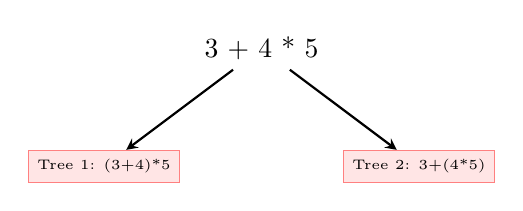
\begin{tikzpicture}[
        tree/.style={rectangle, draw=red!50, fill=red!10, font=\tiny, align=center},
        arrow/.style={->, >=stealth, thick}
    ]
    \node (in) at (0,0) {3 + 4 * 5};
    \node[tree] (t1) at (-2,-1.5) {Tree 1: (3+4)*5};
    \node[tree] (t2) at (2,-1.5) {Tree 2: 3+(4*5)};
    \draw[arrow] (in) -- (t1);
    \draw[arrow] (in) -- (t2);
    \end{tikzpicture}%
    }
    \caption{Ilustrasi ambiguitas grammar}
\end{figure}

\section{Parse Tree dan Abstract Syntax Tree (AST)}

\subsection{Parse Tree (Concrete Syntax Tree)}
Parse Tree adalah representasi visual lengkap dari proses derivasi. Ia mencakup semua detail grammar, termasuk simbol-simbol non-terminal perantara yang mungkin tidak relevan untuk eksekusi program.
\begin{itemize}
    \item \textbf{Kelebihan}: Merefleksikan grammar secara presisi.
    \item \textbf{Kekurangan}: Sangat boros memori dan sulit ditraversasi karena terlalu dalam.
\end{itemize}

\subsection{Abstract Syntax Tree (AST)}
AST adalah versi ringkas dan bersih dari Parse Tree. AST membuang semua token sintaksis yang tidak perlu (seperti kurung \texttt{(}, \texttt{)}, titik koma \texttt{;}, keyword \texttt{then}) dan hanya menyimpan struktur logis operasi.
\begin{itemize}
    \item \textbf{Simpul Dalam}: Operator atau struktur kontrol (\texttt{+}, \texttt{if}, \texttt{while}).
    \item \textbf{Daun}: Operan atau nilai (\texttt{3.14}, \texttt{counter}).
\end{itemize}

\begin{figure}[!htbp]
    \centering
    \adjustbox{max width=0.8\textwidth,center}{%
    \begin{tikzpicture}[
        node/.style={circle, draw=blue!50, fill=blue!10, minimum size=0.8cm, font=\small},
        op/.style={rectangle, draw=red!50, fill=red!10, minimum size=0.8cm, font=\small}
    ]
    % AST for 3 + 4 * 5
    \node[op] (plus) at (0,0) {+};
    \node[node] (n3) at (-1.5,-1.5) {3};
    \node[op] (mul) at (1.5,-1.5) {*};
    \node[node] (n4) at (0.5,-3) {4};
    \node[node] (n5) at (2.5,-3) {5};
    
    \draw[->, thick] (plus) -- (n3);
    \draw[->, thick] (plus) -- (mul);
    \draw[->, thick] (mul) -- (n4);
    \draw[->, thick] (mul) -- (n5);
    
    \node[right=3cm of plus, align=left, font=\footnotesize] {
        \textbf{Struktur Node}:\\
        \texttt{struct Expr \{ ... \};}\\
        \texttt{struct BinOp : Expr \{} \\
        \texttt{  Expr* left;}\\
        \texttt{  Token op;}\\
        \texttt{  Expr* right;}\\
        \texttt{\};}
    };
    \end{tikzpicture}%
    }
    \caption{AST untuk ungkapan $3 + 4 * 5$}
\end{figure}

\section{Integrasi Lexer dan Parser (Bison)}

Parser generator modern seperti \textbf{Bison} bekerja sama dengan \textbf{Flex} melalui mekanisme integrasi token.

\subsection{Mekanisme yylval}
Lexer mengirimkan nilai semantik token (misal: nilai konstanta atau nama variabel) ke parser melalui variabel global \texttt{yylval}.

\subsection{Struktur File Bison (.y)}
\begin{lstlisting}[language=C]
%token NUMBER IDENTIFIER
%left '+' '-'
%left '*' '/'
%%
expr: expr '+' expr | NUMBER ;
%%
\end{lstlisting}

\begin{figure}[!htbp]
    \centering
    \adjustbox{max width=0.8\textwidth,center}{%
    \begin{tikzpicture}[
        box/.style={rectangle, draw=blue!50, fill=blue!10, font=\tiny, align=center},
        arrow/.style={->, >=stealth, thick}
    ]
    \node[box] (flex) {Flex (Lexer)};
    \node[box, right=2cm of flex] (bison) {Bison (Parser)};
    \draw[arrow] (flex) -- node[above, font=\tiny] {Tokens + yylval} (bison);
    \end{tikzpicture}%
    }
    \caption{Integrasi data antara Flex dan Bison}
\end{figure}

\section{Implementasi: Hand-written Recursive Descent}

Recursive Descent adalah teknik parsing paling populer untuk implementasi manual karena struktur kodenya sangat mirip dengan grammar EBNF-nya.

\subsection{Pola Implementasi}
Setiap aturan produksi diterjemahkan menjadi satu fungsi.
\begin{itemize}
    \item \textbf{Pilihan ($\mid$)}: Menjadi \texttt{if-else} atau \texttt{switch-case}.
    \item \textbf{Repetisi ($*$ atau $+$)}: Menjadi \texttt{while} atau \texttt{do-while} loop.
    \item \textbf{Sequence}: Menjadi pemanggilan fungsi berurutan.
\end{itemize}

\subsection{Pratt Parsing (Top-Down Operator Precedence)}
Recursive Descent menjadi agak berbelit saat menangani ekspresi matematika dengan banyak level presedensi (misal: 10 level dari $||$ hingga $()$). Kita harus membuat 10 fungsi bersarang (\texttt{parseOr}, \texttt{parseAnd}, ..., \texttt{parsePrimary}).

Sebagai alternatif, teknik \textbf{Pratt Parsing} (digunakan di Python dan Rust) menggunakan tabel lookup untuk presedensi.
\begin{lstlisting}[language=C++]
// Konsep Pratt Parsing
Expression parsePratt(int precedence) {
    Token t = advance();
    Expression left = prefixParselet[t.type].parse(t);
    while (precedence < getPrecedence(peek().type)) {
        t = advance();
        left = infixParselet[t.type].parse(left, t);
    }
    return left;
}
\end{lstlisting}
Teknik ini jauh lebih ringkas untuk ekspresi, namun Recursive Descent tetap lebih unggul untuk statement (\texttt{if}, \texttt{while}, \texttt{class}).

\section{Precedence dan Error Recovery}

\subsection{Menangani Operator Precedence}
Dalam \textit{Recursive Descent}, precedence diatur secara implisit melalui struktur fungsi yang berlapis. Fungsi yang dipanggil paling dalam (misal: \texttt{parseFactor}) memiliki prioritas eksekusi paling tinggi (mengikat operan lebih kuat).
\begin{itemize}
    \item \textbf{Lowest Precedence}: \texttt{parseExpression} (menangani \texttt{+ -}).
    \item \textbf{Medium Precedence}: \texttt{parseTerm} (menangani \texttt{* /}).
    \item \textbf{Highest Precedence}: \texttt{parseFactor} (menangani \texttt{( )}, angka, variabel).
\end{itemize}

\subsection{Error Recovery: Panic Mode}
Parser yang baik tidak boleh berhenti (\textit{abort}) begitu menemukan satu kesalahan sintaks.
\begin{enumerate}
    \item \textbf{Deteksi Error}: Parser menemukan token tak terduga (misal: \texttt{Expected ';'}).
    \item \textbf{Masuk Mode Panik}: Parser membuang semua produksi yang sedang dikerjakan.
    \item \textbf{Sinkronisasi}: Parser terus membuang token input (\textit{eating tokens}) sampai menemukan token "jangkar" yang aman, biasanya titik koma (\texttt{;}) atau kurung kurawal tutup (\texttt{\}}).
\end{enumerate}

\begin{lstlisting}[language=C++]
void Parser::panic() {
    while (!isAtEnd()) {
        if (previous().type == SEMICOLON) return;
        switch (peek().type) {
            case CLASS: case FUN: case VAR: case FOR: case IF: return;
        }
        advance();
    }
}
\end{lstlisting}

\section{Bottom-Up Parsing: Shift-Reduce dan LR}

\subsection{Konsep Shift-Reduce}
Bottom-up parsing bekerja dengan dua operasi utama:
\begin{itemize}
    \item \textbf{Shift}: Memindahkan token dari input ke stack.
    \item \textbf{Reduce}: Mengganti simbol di puncak stack yang cocok dengan \textit{handle} (RHS sebuah produksi) menjadi non-terminal (LHS).
\end{itemize}

\subsection{LR Parsing}
LR parsing ($L$: Left-to-right, $R$: Rightmost derivation in reverse) adalah metode yang paling powerful. Varian LR meliputi:
\begin{itemize}
    \item \textbf{SLR(1)}: Simple LR, menggunakan \textit{Follow set} dasar.
    \item \textbf{LALR(1)}: Look-Ahead LR, standar industri (digunakan Bison/Yacc).
    \item \textbf{Canonical LR(1)}: Paling powerful namun membutuhkan tabel sangat besar.
\end{itemize}

\begin{figure}[!htbp]
    \centering
    \adjustbox{max width=0.8\textwidth,center}{%
    \begin{tikzpicture}[
        stack/.style={rectangle, draw=green!50, fill=green!10, font=\tiny, align=center},
        arrow/.style={->, >=stealth, thick}
    ]
    \node[stack] (s) {Stack Content};
    \node[right=of s, font=\tiny] (la) {Lookahead Token};
    \node[below=1cm of s, font=\tiny] (table) {Action/Goto Table};
    \draw[arrow] (s) -- (table);
    \draw[arrow] (la) -- (table);
    \end{tikzpicture}%
    }
    \caption{Model konseptual LR Parser}
\end{figure}

\section{Parser Generator: Bison Deep Dive}

\subsection{Shift/Reduce Conflict}
Konflik ini terjadi ketika parser bingung memilih antara menggeser (\textit{shift}) token baru atau mereduksi (\textit{reduce}) stack sekarang.
Contoh klasik: \texttt{if E1 then if E2 then S1 else S2}.
Di sini, parser memiliki \texttt{if E then S} di stack dan melihat \texttt{else}.
\begin{itemize}
    \item \textbf{Shift}: Membawa \texttt{else} masuk (berarti \texttt{else} milik \texttt{if} dalam).
    \item \textbf{Reduce}: Mengubah \texttt{if E then S} menjadi \textit{Stmt} (berarti \texttt{else} milik \texttt{if} luar).
\end{itemize}
Default Bison adalah \textbf{Shift} (yang benar untuk kasus ini).

\subsection{Operator Precedence Declarations}
Tanpa mengubah grammar menjadi rumit, kita bisa memberi tahu Bison prioritas operator:
\begin{lstlisting}[language=C]
%left '+' '-'   // Precedence rendah, asosiasi kiri
%left '*' '/'   // Precedence tinggi, asosiasi kiri
%right '^'      // Precedence lebih tinggi, asosiasi kanan
%nonassoc UMINUS // Untuk operator unary minus
\end{lstlisting}
Aturan yang dideklarasikan lebih bawah memiliki precedence lebih tinggi.

\subsection{Error Handling dengan Token 'error'}
Bison memiliki token spesial \texttt{error} untuk pemulihan.
\begin{lstlisting}[language=C]
stmt: 
    expr ';' 
  | error ';' { yyerror("Syntax error, skipping to semicolon"); yyerrok; }
;
\end{lstlisting}
Jika terjadi kesalahan dalam \textit{stmt}, parser akan membuang token sampai menemukan titik koma, lalu mengeksekusi aksi pemulihan, dan melanjutkan parsing seolah-olah tidak ada masalah.


% ============================================================
% AKTIVITAS PEMBELAJARAN
% ============================================================
\begin{aktivitas}
  \item \textbf{Grammar Design}: Buat CFG untuk bahasa ekspresi aritmatika sederhana.
  \item \textbf{LL(1) Conversion}: Konversi grammar dengan left recursion ke LL(1).
  \item \textbf{Recursive Descent}: Implementasikan recursive descent parser untuk kalkulator.
  \item \textbf{Bison Practice}: Buat parser untuk bahasa dengan assignment dan control flow.
  \item \textbf{Error Recovery}: Implementasikan panic mode recovery dalam parser Anda.
\end{aktivitas}

% ============================================================
% LATIHAN DAN REFLEKSI
% ============================================================
\begin{latihan}
  \item Identifikasi apakah grammar berikut LL(1): $S \rightarrow aSb | \epsilon$!
  \item Hapus left recursion dari grammar: $E \rightarrow E + T | T$!
  \item Buat recursive descent parser untuk grammar: $S \rightarrow (S)S | \epsilon$!
  \item Jelaskan perbedaan antara SLR(1) dan LALR(1) parser!
  \item Implementasikan error recovery with panic mode untuk parser Anda!
  \item \textbf{Refleksi}: Konsep parsing mana yang paling sulit dan bagaimana cara memahaminya?
\end{latihan}

% ============================================================
% ASESMEN
% ============================================================
\begin{asesmen}
\textbf{Instrumen Penilaian untuk Sub-CPMK 2.3-2.4}

\textbf{A. Pilihan Ganda}

\begin{enumerate}
  \item Grammar dengan left recursion TIDAK cocok untuk:
  \begin{enumerate}
    \item LL(1) parser
    \item LR(1) parser
    \item Recursive descent parser
    \item Top-down parser
  \end{enumerate}
  
  \item Tool yang digunakan untuk generate LR parser adalah:
  \begin{enumerate}
    \item Flex
    \item Bison
    \item Make
    \item GCC
  \end{enumerate}
  
  \item Lookahead dalam LL(1) berarti:
  \begin{enumerate}
    \item 1 token lookahead
    \item 1 character lookahead
    \item 1 production lookahead
    \item 1 derivation lookahead
  \end{enumerate}
\end{enumerate}

\textbf{B. Essay}

\begin{enumerate}
  \item Jelaskan langkah-langkah mengkonversi grammar dengan left recursion ke LL(1)!
  \item Desain dan implementasikan parser untuk bahasa dengan variabel assignment dan arithmetic expressions!
\end{enumerate}

\textbf{Rubrik Penilaian}: Lihat Lampiran A
\end{asesmen}

% ============================================================
% CHECKLIST KOMPETENSI
% ============================================================
\begin{checklist}
  \item Saya dapat membangun recursive descent parser untuk grammar LL(1)
  \item Saya dapat menggunakan parser generator (Flex/Bison) untuk bahasa sederhana
  \item Saya dapat mengidentifikasi apakah suatu grammar LL(1)
  \item Saya dapat menghapus left recursion dari grammar
  \item Saya dapat mengimplementasikan error recovery dalam parser
  \item Saya memahami perbedaan top-down dan bottom-up parsing
\end{checklist}

% ============================================================
% RANGKUMAN
% ============================================================
\begin{rangkuman}
Bab ini membahas parsing dan syntax analysis, termasuk CFG, LL(1) parsing, recursive descent, LR parsing, dan parser generator tools. Mahasiswa belajar membangun parser manual dan menggunakan tools modern.

\textbf{Poin Kunci:}
\begin{itemize}
  \item Parser memverifikasi sintaks dan membangun parse tree dari token stream
  \item LL(1) grammar cocok untuk recursive descent parser
  \item LR parser lebih powerful tapi lebih kompleks
  \item Parser generator (Bison) otomatisasi pembuatan parser dari grammar
  \item Error recovery penting untuk parser yang robust
\end{itemize}

\textbf{Kata Kunci}: \compiler{Parsing}, \compiler{CFG}, \compiler{LL(1)}, \compiler{Recursive Descent}, \compiler{LR Parser}, \compiler{Bison}, \compiler{Syntax Analysis}, \compiler{Error Recovery}
\end{rangkuman}

\ifSubfilesClassLoaded{%
    \clearpage
    \printbibliography[title={Daftar Pustaka}]
    \end{refsection}
}{}

\end{document}
